\chapter{Experiments and Results}
\label{chap:experiments-results}

\section{Introduction}

This chapter presents the experiments and results for the language-guided active view selection system. The aim is to evaluate whether CLIP-based selection, a learned MLP reranker, and a trained active view selector can improve instruction-relevant view prediction under limited observation budgets.

Two datasets are used: the shuffled CO3D multi-view instruction set and the UMD+GT affordance view-selection set. Methods are compared under budgets \(k \in \{1,2,3,4,5\}\). The main UMD+GT comparison uses 20 random-initial trials with mean \(\pm\) standard deviation; CO3D results and ablations use 10 trials. Ablation studies measure each component's gain relative to a shared random-plus-CLIP baseline.

\section{Experimental Setup}

Unless otherwise stated, all methods start from a random initial view. Additional views are selected until the budget is reached, after which the observed views are reranked and the top-1 view is returned. A prediction is correct if that view belongs to the ground-truth set.

The compared methods, matching the legend labels used in the figures, are:

\begin{itemize}
    \item \textbf{Random}: select additional views uniformly at random; rank the observed set with CLIP cosine similarity.
    \item \textbf{Exhaustive CLIP}: score all five candidate views with CLIP and return the global top-1 view (no sequential budget constraint).
    \item \textbf{Active policy}: CLIP relevance-plus-novelty sequential selection, then CLIP ranking of the observed set.
    \item \textbf{Learned reranker}: random additional views, then a trained MLP ranks the observed set.
    \item \textbf{Trained active + CLIP}: a trained MLP selector chooses the next views; CLIP ranks the observed set.
    \item \textbf{Trained active + learned reranker}: full pipeline with trained selection and trained final ranking.
\end{itemize}

On CO3D, models are trained on objects 16--30, validated on objects 11--15, and evaluated on objects 1--10. On UMD+GT, the official instance split is used, with a held-out validation subset of the training tools. Grouping is by object category on CO3D and by affordance on UMD+GT.

\section{CO3D Results}

\subsection{Main Method Comparison}

Table~\ref{tab:co3d-budget-results} reports mean accuracy on the shuffled CO3D evaluation set. Because views are shuffled, budget~1 no longer benefits from first-view bias: all sequential methods start near 0.30--0.31, which is close to random chance given the number of ground-truth views per sample.

\begin{table}[htbp]
    \centering
    \caption{Accuracy on the shuffled CO3D evaluation set under different observation budgets.}
    \label{tab:co3d-budget-results}
    \footnotesize
    \setlength{\tabcolsep}{4pt}
    \begin{tabular}{lccccc}
        \toprule
        Method & B1 & B2 & B3 & B4 & B5 \\
        \midrule
        Random + CLIP & 0.300 & 0.300 & 0.310 & 0.300 & 0.300 \\
        Exhaustive CLIP & 0.360 & 0.360 & 0.360 & 0.360 & 0.360 \\
        Active policy + CLIP & 0.306 & 0.348 & 0.356 & 0.360 & 0.360 \\
        Random + learned reranker & 0.306 & 0.416 & 0.478 & 0.498 & 0.520 \\
        Trained active + CLIP & 0.306 & 0.386 & 0.344 & 0.368 & 0.360 \\
        Trained active + learned reranker & 0.306 & \textbf{0.534} & \textbf{0.520} & \textbf{0.520} & \textbf{0.520} \\
        \bottomrule
    \end{tabular}
\end{table}

\begin{figure}[htbp]
    \centering
    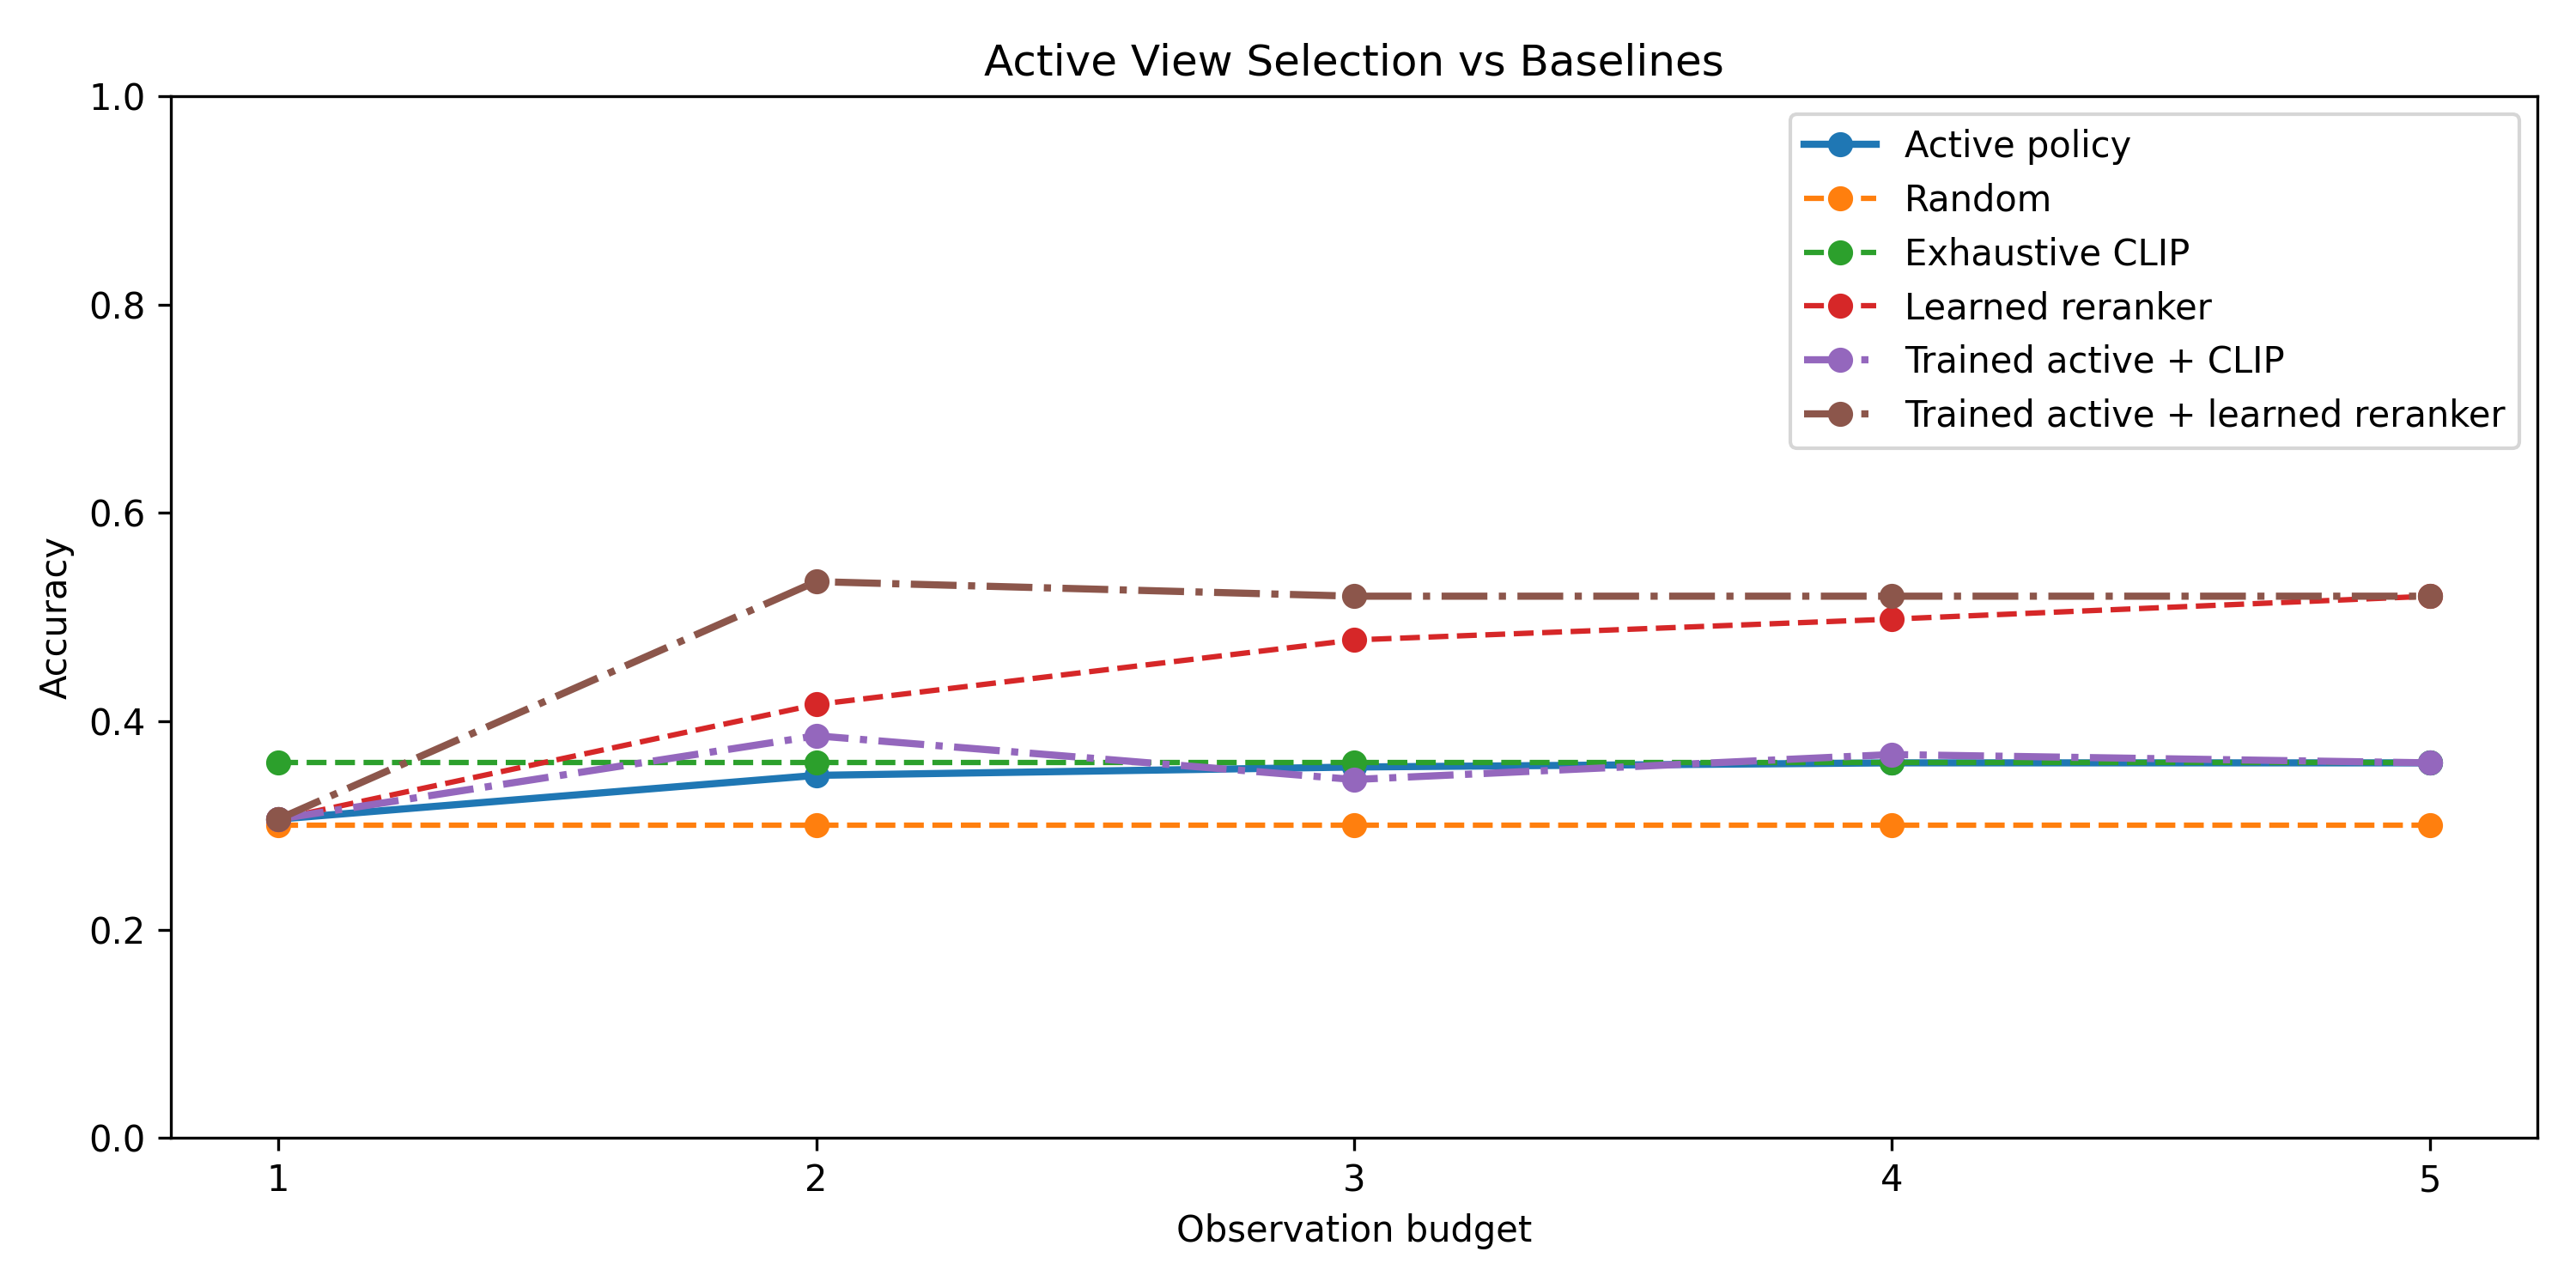
\includegraphics[width=0.95\textwidth]{figures/co3d_method_comparison_vs_budget.png}
    \caption{CO3D method comparison on the shuffled evaluation set.
    \textbf{Active policy}: CLIP relevance+novelty selection with CLIP final ranking.
    \textbf{Random}: random additional views with CLIP ranking.
    \textbf{Exhaustive CLIP}: global CLIP top-1 over all five views.
    \textbf{Learned reranker}: random selection with MLP final ranking.
    \textbf{Trained active + CLIP}: trained MLP selector with CLIP ranking.
    \textbf{Trained active + learned reranker}: trained selector with MLP ranking (full pipeline).}
    \label{fig:co3d-method-comparison}
\end{figure}

Figure~\ref{fig:co3d-method-comparison} visualises the same comparison. Three findings stand out.

First, CLIP-only methods remain close to exhaustive CLIP. The relevance-plus-novelty active policy reaches about 0.35--0.36 for budgets 2--5, only marginally above the random-plus-CLIP baseline and similar to exhaustive CLIP at 0.36. Language-guided CLIP scoring is therefore better than non-semantic selection, but the heuristic active policy does not clearly beat direct CLIP ranking.

Second, the learned reranker is the main source of improvement. With random selection, learned reranking rises from 0.306 at budget~1 to 0.478 at budget~3 and 0.520 at budget~5. This shows that a lightweight MLP can adapt frozen CLIP features to the instruction-specific ground-truth labels much more effectively than cosine similarity alone.

Third, the full pipeline is strongest at low budgets. At budget~2, trained selection plus learned reranking reaches 0.534, compared with 0.416 for learned reranking alone. By budget~5, both learned-reranker methods converge to 0.520 because the observed set contains all five views and only the final ranking matters.

\begin{figure}[htbp]
    \centering
    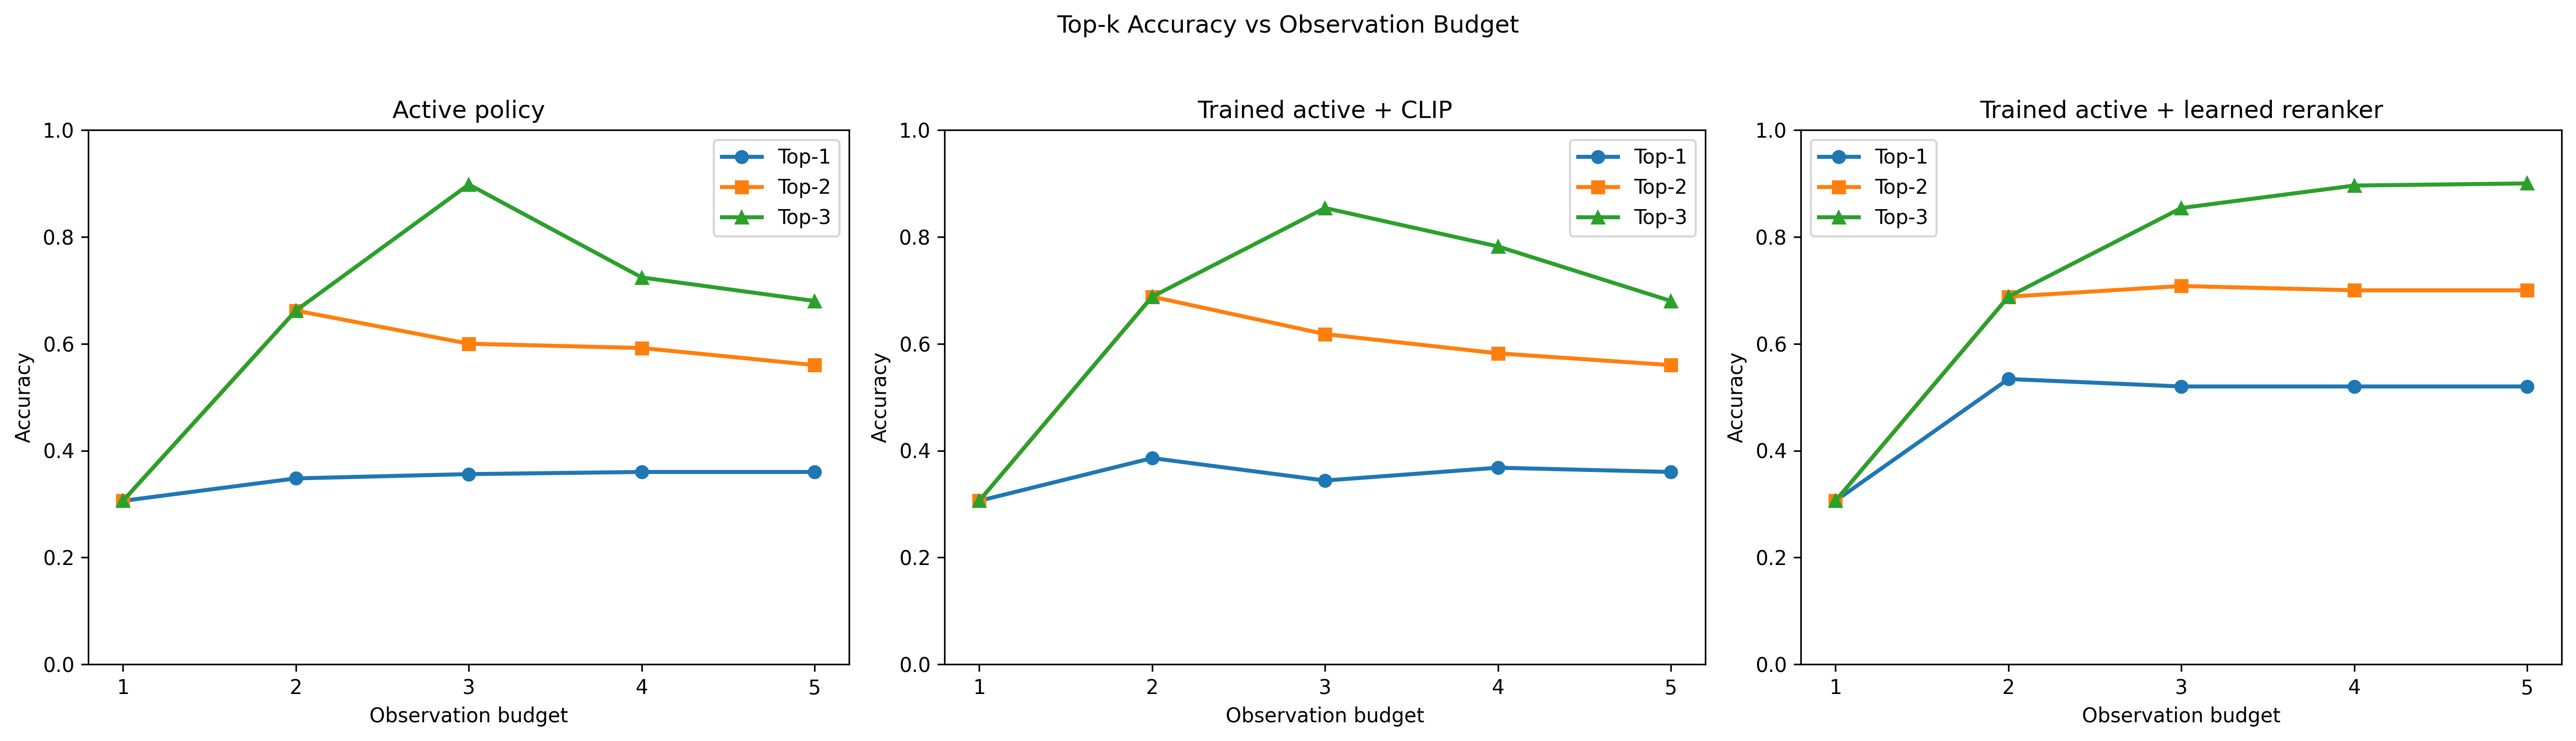
\includegraphics[width=0.95\textwidth]{figures/co3d_topk_vs_budget.png}
    \caption{CO3D Top-\(k\) accuracy versus budget for the active policy.
    Top-1 is the final predicted view; Top-2/Top-3 succeed if any of the highest-ranked observed views is ground truth.}
    \label{fig:co3d-topk}
\end{figure}

Figure~\ref{fig:co3d-topk} shows Top-1, Top-2, and Top-3 accuracy. Top-2 and Top-3 are consistently higher than Top-1, indicating that correct views are often ranked near the top even when they are not selected as the final answer. This supports the interpretation that ranking quality is the central bottleneck, and that learned reranking addresses it directly.

\subsection{CO3D Ablation}

Figure~\ref{fig:co3d-ablation-budget3} and Table~\ref{tab:co3d-ablation-budget3} report accuracy gains versus the random-plus-CLIP baseline at budget~3. Validation accuracy was 0.80 for the reranker and 0.76 for the selector.

\begin{figure}[htbp]
    \centering
    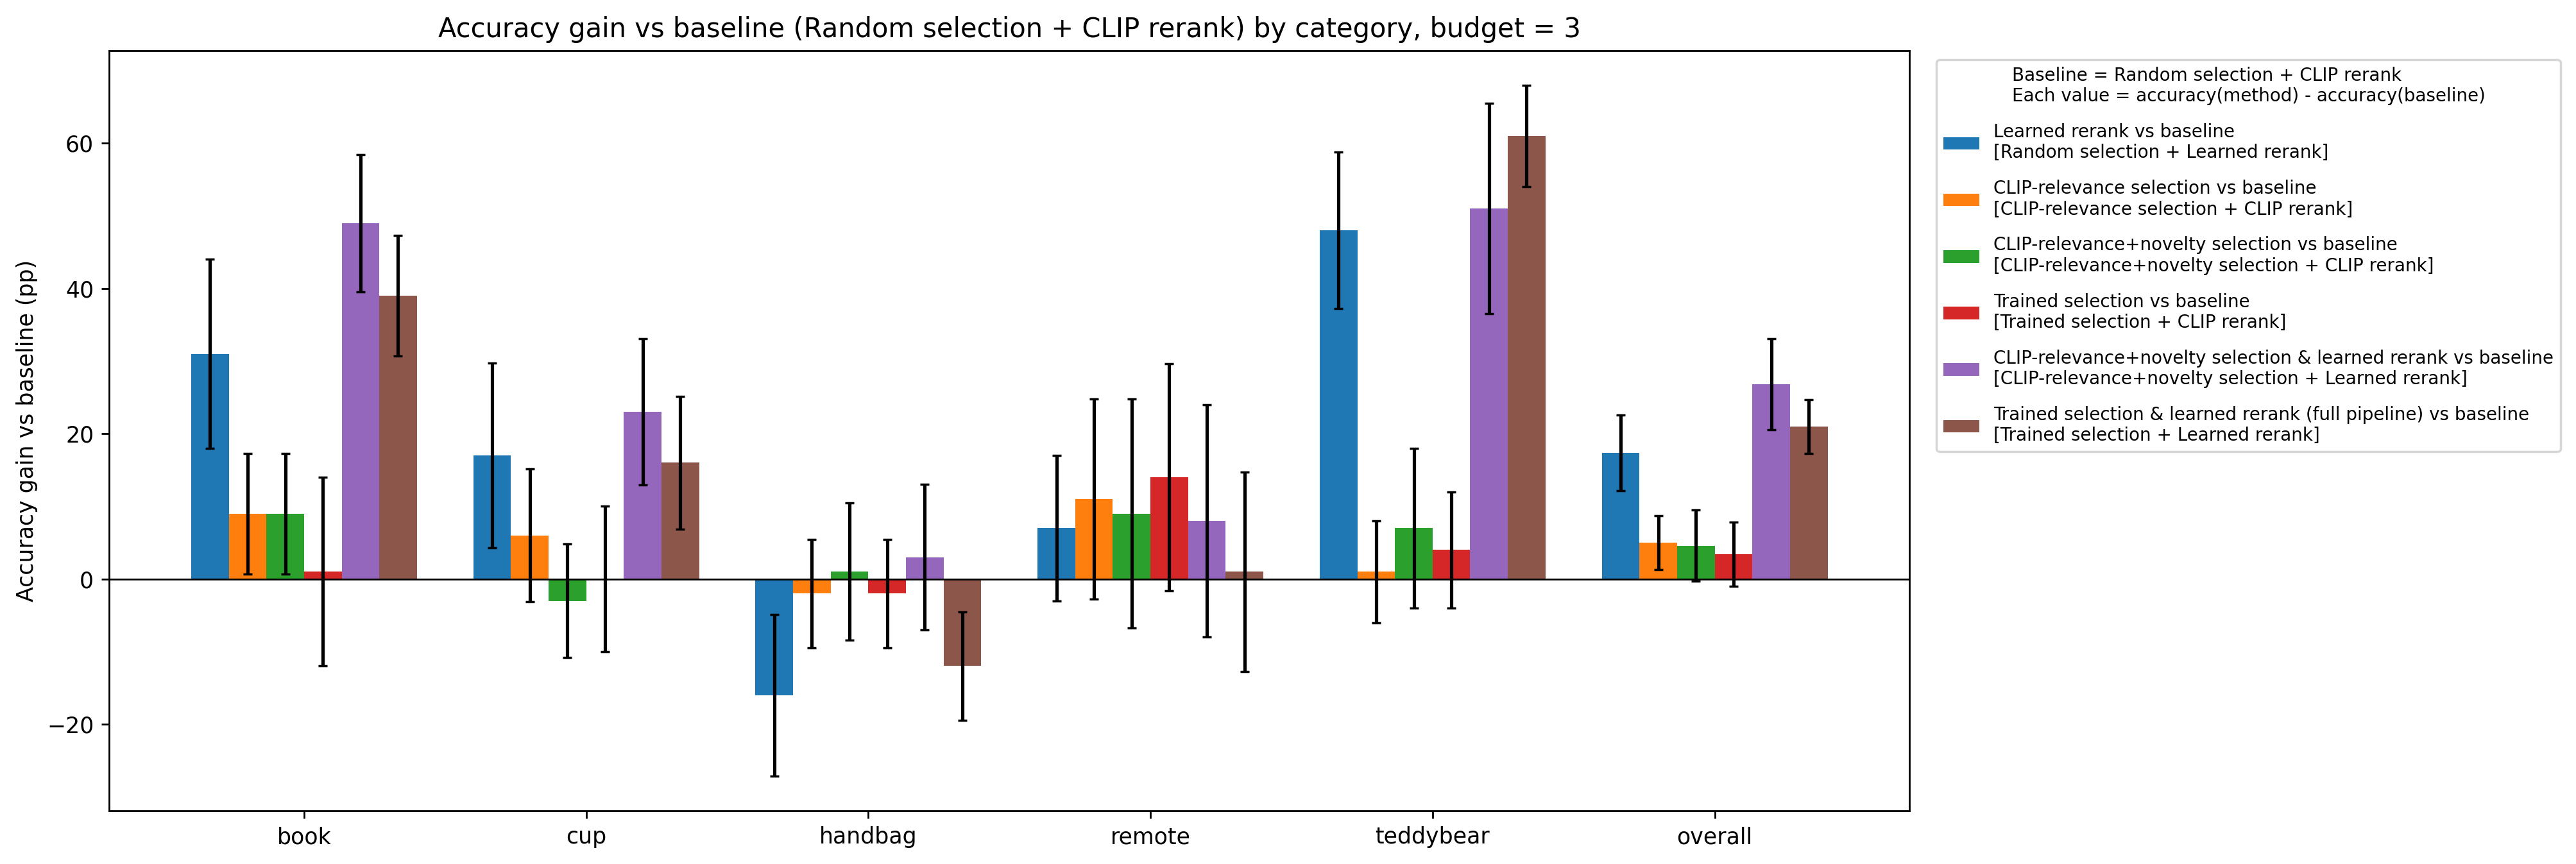
\includegraphics[width=0.95\textwidth]{figures/co3d_component_gain_budget_3.png}
    \caption{CO3D ablation at budget~3.
    Each bar is accuracy(method)~$-$~accuracy(random selection + CLIP rerank).
    Legend entries name the component being added or replaced relative to that shared baseline
    (for example, learned rerank only, selection-only variants, and the full trained pipeline).}
    \label{fig:co3d-ablation-budget3}
\end{figure}

\begin{table}[htbp]
    \centering
    \caption{CO3D accuracy gain versus random+CLIP at budget~3 (percentage points).}
    \label{tab:co3d-ablation-budget3}
    \footnotesize
    \setlength{\tabcolsep}{3.5pt}
    \begin{tabular}{lrrrrrr}
        \toprule
        Comparison & book & cup & bag & rem. & teddy & all \\
        \midrule
        Learned rerank & +31.0 & +17.0 & $-$16.0 & +7.0 & +48.0 & +17.4 \\
        CLIP-relevance selection & +9.0 & +6.0 & $-$2.0 & +11.0 & +1.0 & +5.0 \\
        CLIP-rel+novelty selection & +9.0 & $-$3.0 & +1.0 & +9.0 & +7.0 & +4.6 \\
        Trained selection & +1.0 & 0.0 & $-$2.0 & +14.0 & +4.0 & +3.4 \\
        CLIP-rel+nov + learned & +49.0 & +23.0 & +3.0 & +8.0 & +51.0 & +26.8 \\
        Full pipeline & +39.0 & +16.0 & $-$12.0 & +1.0 & +61.0 & +21.0 \\
        \bottomrule
    \end{tabular}
\end{table}

The ablation confirms that learned reranking drives most of the gain. Selection-only methods add only about 3--5 overall points. Interestingly, CLIP relevance-plus-novelty selection combined with learned reranking (+26.8 overall) slightly outperforms the full trained pipeline (+21.0). This suggests that on CO3D the novelty term can supply complementary views to the reranker, whereas the trained selector, which is trained with the same GT-view objective as the reranker, tends to fetch views that the reranker already likes. Category-level results are noisy because each category has only 10 evaluation objects; handbag in particular is negative for several learned-reranker configurations.

\begin{figure}[htbp]
    \centering
    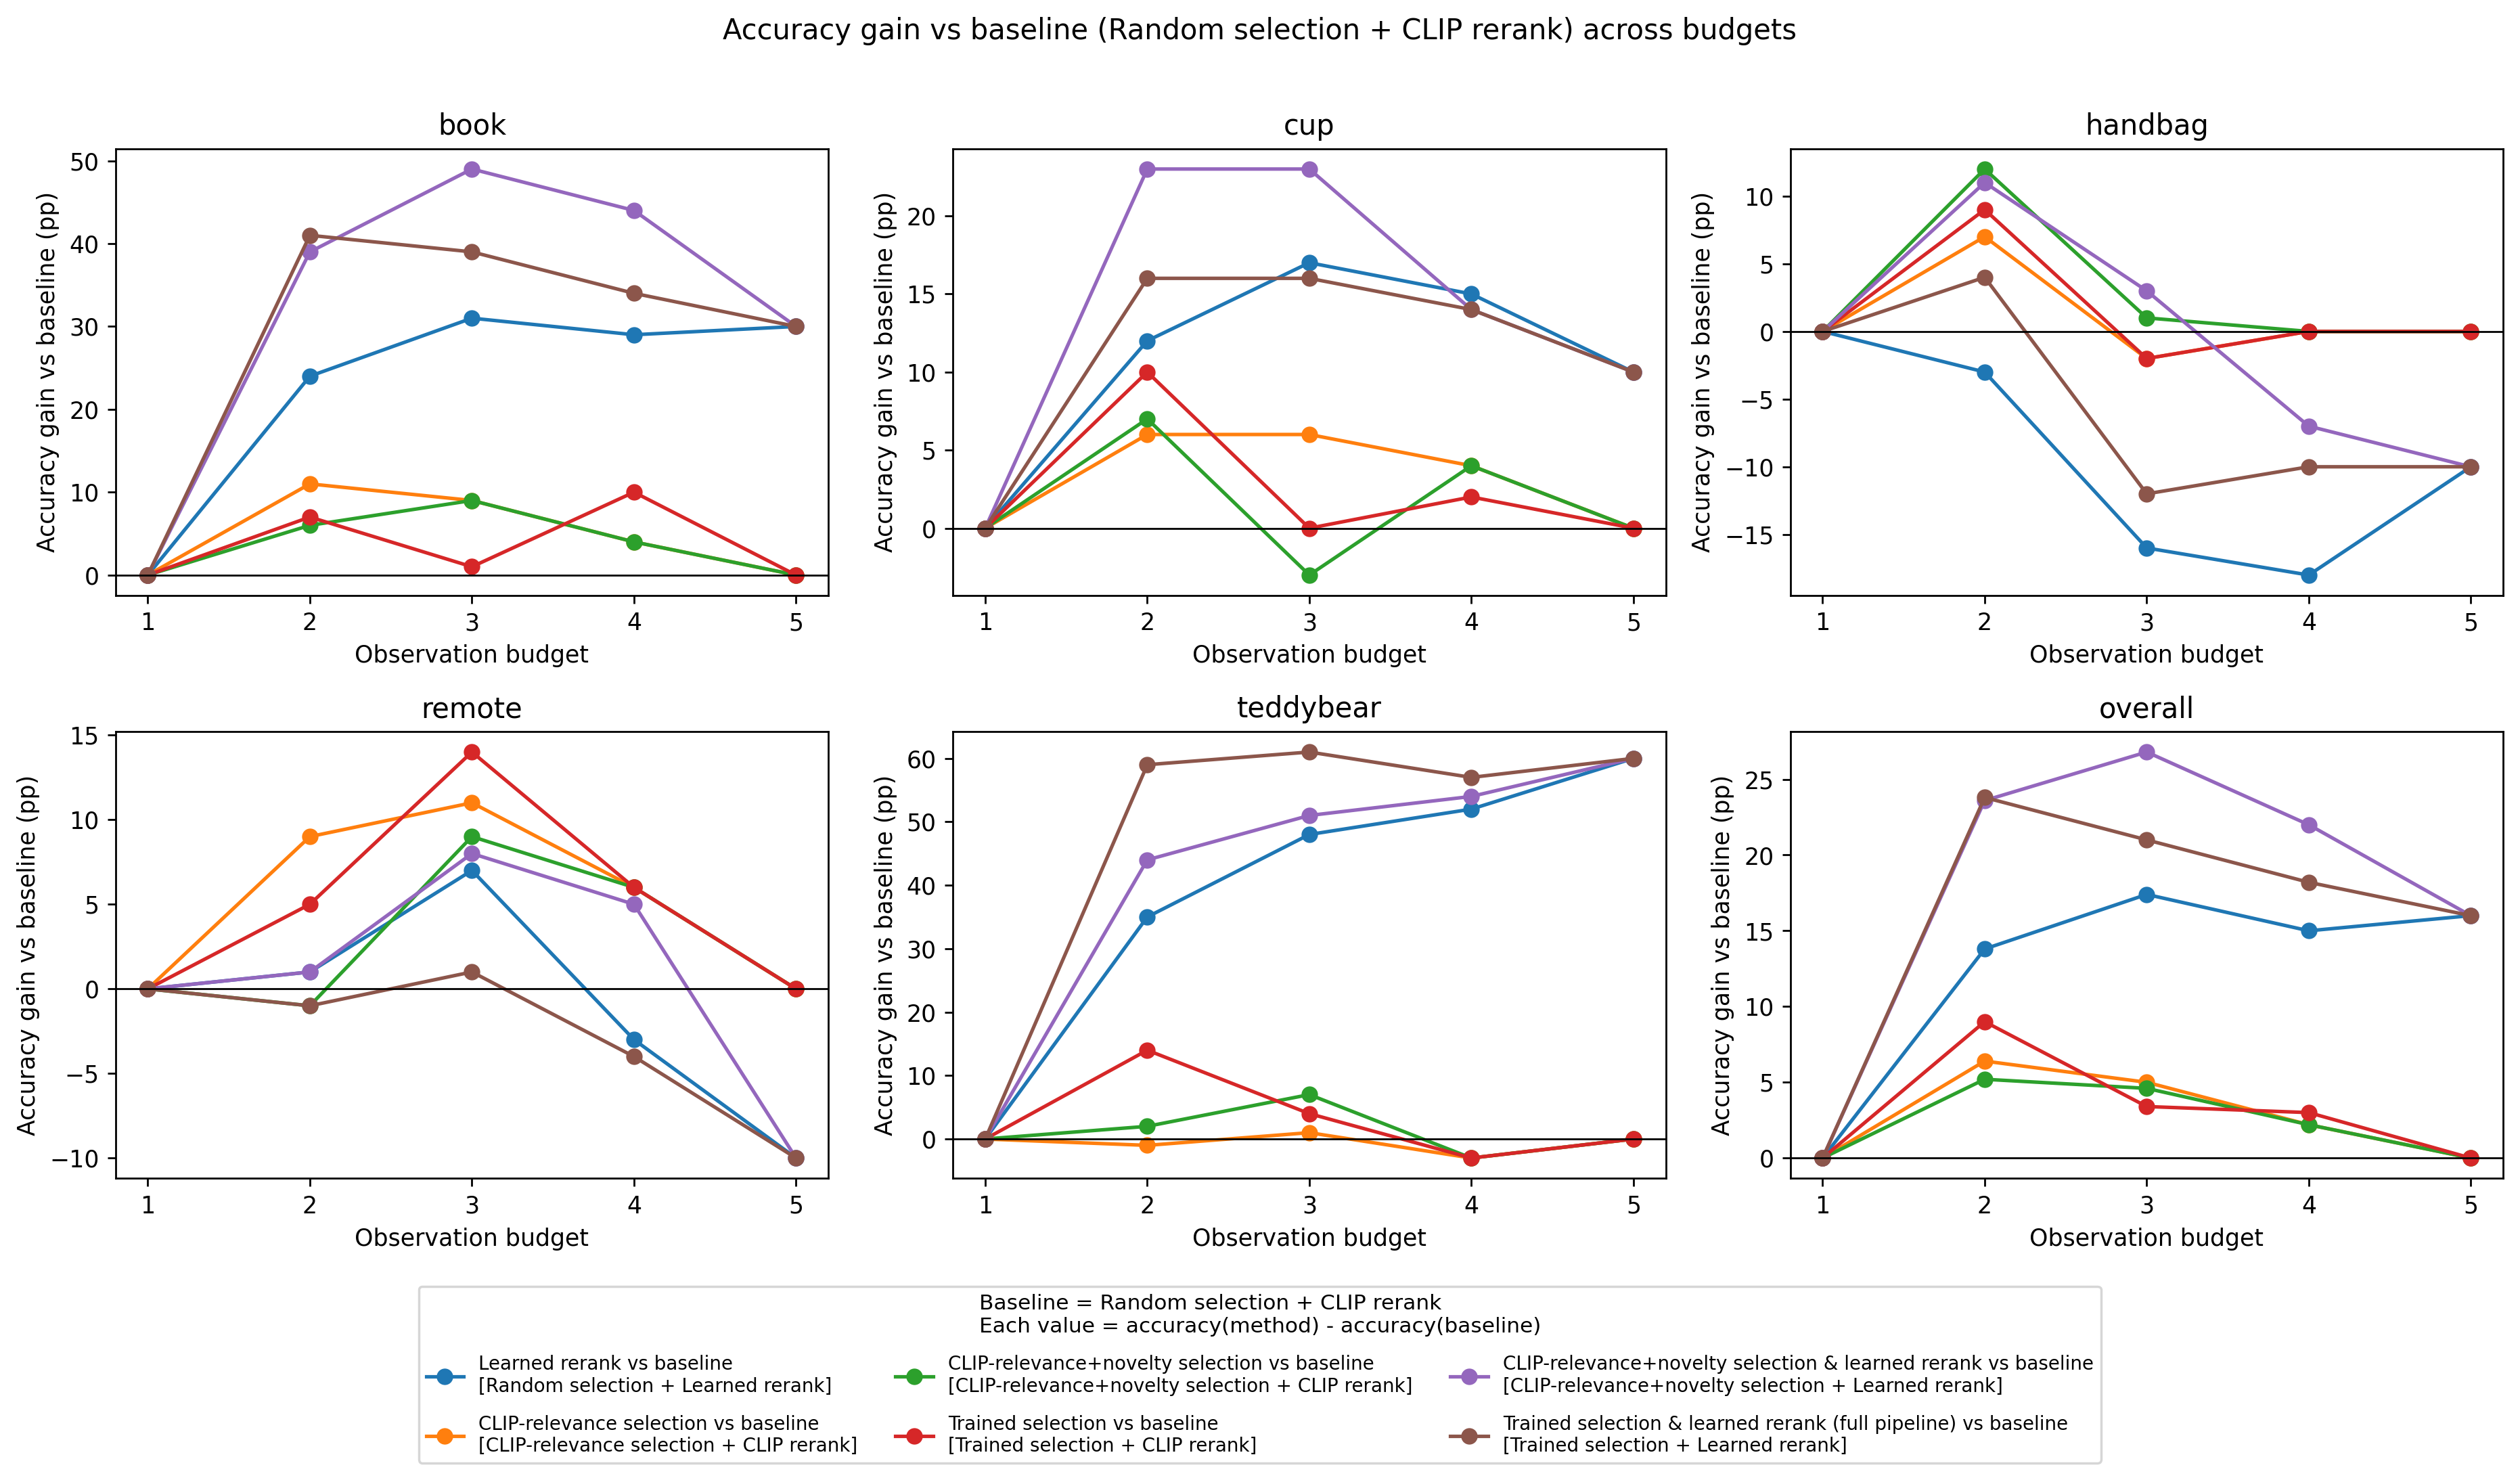
\includegraphics[width=0.95\textwidth]{figures/co3d_component_gain_vs_budget.png}
    \caption{CO3D component gains versus budget.
    Every curve is accuracy(method)~$-$~accuracy(random+CLIP), so positive values mean improvement over the shared baseline.
    Curves correspond to the same component definitions as in Figure~\ref{fig:co3d-ablation-budget3}.}
    \label{fig:co3d-ablation-vs-budget}
\end{figure}

\section{UMD+GT Results}

\subsection{Main Method Comparison}

Table~\ref{tab:umd-budget-results} reports mean accuracy on the UMD+GT test set over 20 random-initial trials.
The random-plus-CLIP baseline is about 0.46--0.47, close to the random-pick chance of 0.43 arising from multiple ground-truth views per sample.
Exhaustive CLIP reaches only 0.481, showing that cosine similarity alone is a weak final ranker for affordance-view instructions.

\begin{table}[htbp]
    \centering
    \caption{UMD+GT mean accuracy over 20 trials.
    Stochastic methods share the same random-initial seeds; values are means (standard deviations appear as error bars in Figure~\ref{fig:umd-method-comparison}).
    At budget~5 the observed set contains all views, so trial variance collapses to zero.}
    \label{tab:umd-budget-results}
    \footnotesize
    \setlength{\tabcolsep}{3.5pt}
    \begin{tabular}{lccccc}
        \toprule
        Method & B1 & B2 & B3 & B4 & B5 \\
        \midrule
        Random + CLIP & 0.439 & 0.465 & 0.462 & 0.473 & 0.481 \\
        Exhaustive CLIP & 0.481 & 0.481 & 0.481 & 0.481 & 0.481 \\
        Active policy + CLIP & 0.439 & 0.457 & 0.473 & 0.484 & 0.481 \\
        Random + learned reranker & 0.439 & 0.571 & 0.632 & 0.674 & 0.696 \\
        Trained active + CLIP & 0.439 & 0.524 & 0.508 & 0.496 & 0.481 \\
        Trained active + learned reranker & 0.439 & \textbf{0.669} & \textbf{0.680} & \textbf{0.693} & \textbf{0.696} \\
        \bottomrule
    \end{tabular}
\end{table}

\begin{figure}[htbp]
    \centering
    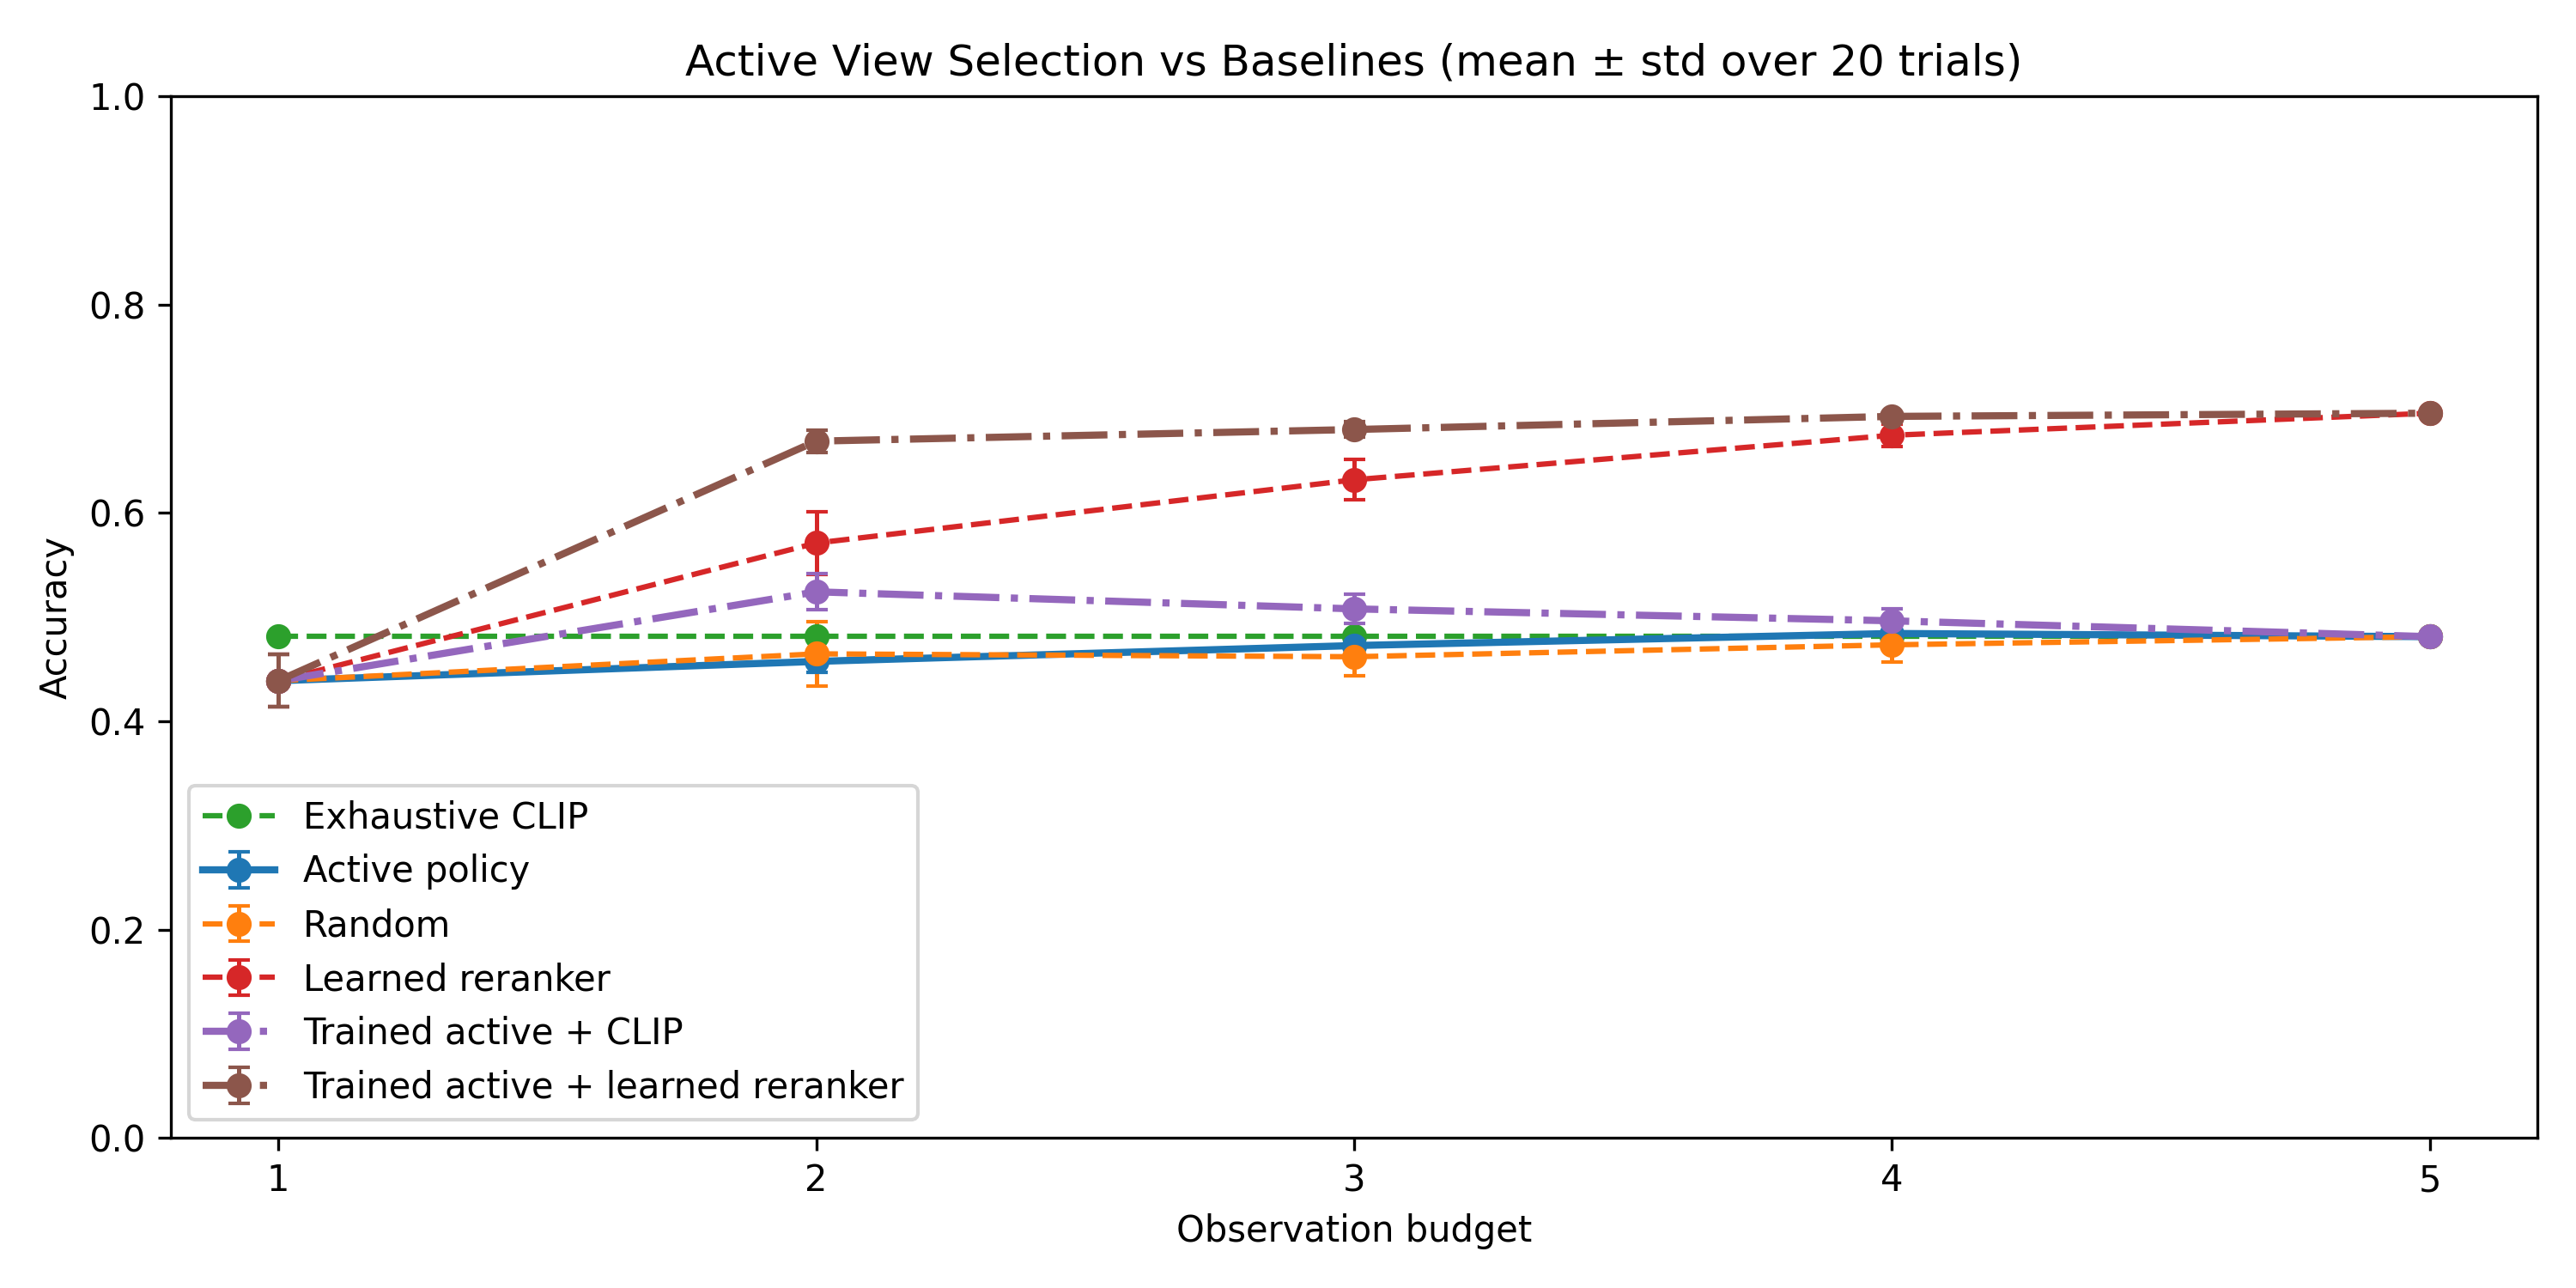
\includegraphics[width=0.95\textwidth]{figures/umd_method_comparison_vs_budget.png}
    \caption{UMD+GT method comparison with mean \(\pm\) std over 20 trials.
    \textbf{Active policy}: CLIP relevance+novelty selection, CLIP final ranking.
    \textbf{Random}: random additional views, CLIP ranking.
    \textbf{Exhaustive CLIP}: global CLIP top-1 over all views (deterministic; no error bar).
    \textbf{Learned reranker}: random selection, MLP final ranking.
    \textbf{Trained active + CLIP}: trained MLP selector, CLIP ranking.
    \textbf{Trained active + learned reranker}: full pipeline (trained selector + MLP ranking).}
    \label{fig:umd-method-comparison}
\end{figure}

On UMD+GT, the full pipeline is clearly the strongest method at low and medium budgets.
At budget~2 it already reaches \(0.669 \pm 0.011\), while learned reranking alone is \(0.571 \pm 0.030\) and needs about four views to approach the full pipeline.
Validation accuracy was 0.744 for the reranker and 0.705 for the selector.

Unlike CO3D, the trained selector provides a clear low-budget benefit when paired with the learned reranker.
A likely reason is that UMD turntable sequences change affordance visibility smoothly with viewpoint, giving the selector a more consistent signal for which unobserved view is likely to be a ground-truth view.

\begin{figure}[htbp]
    \centering
    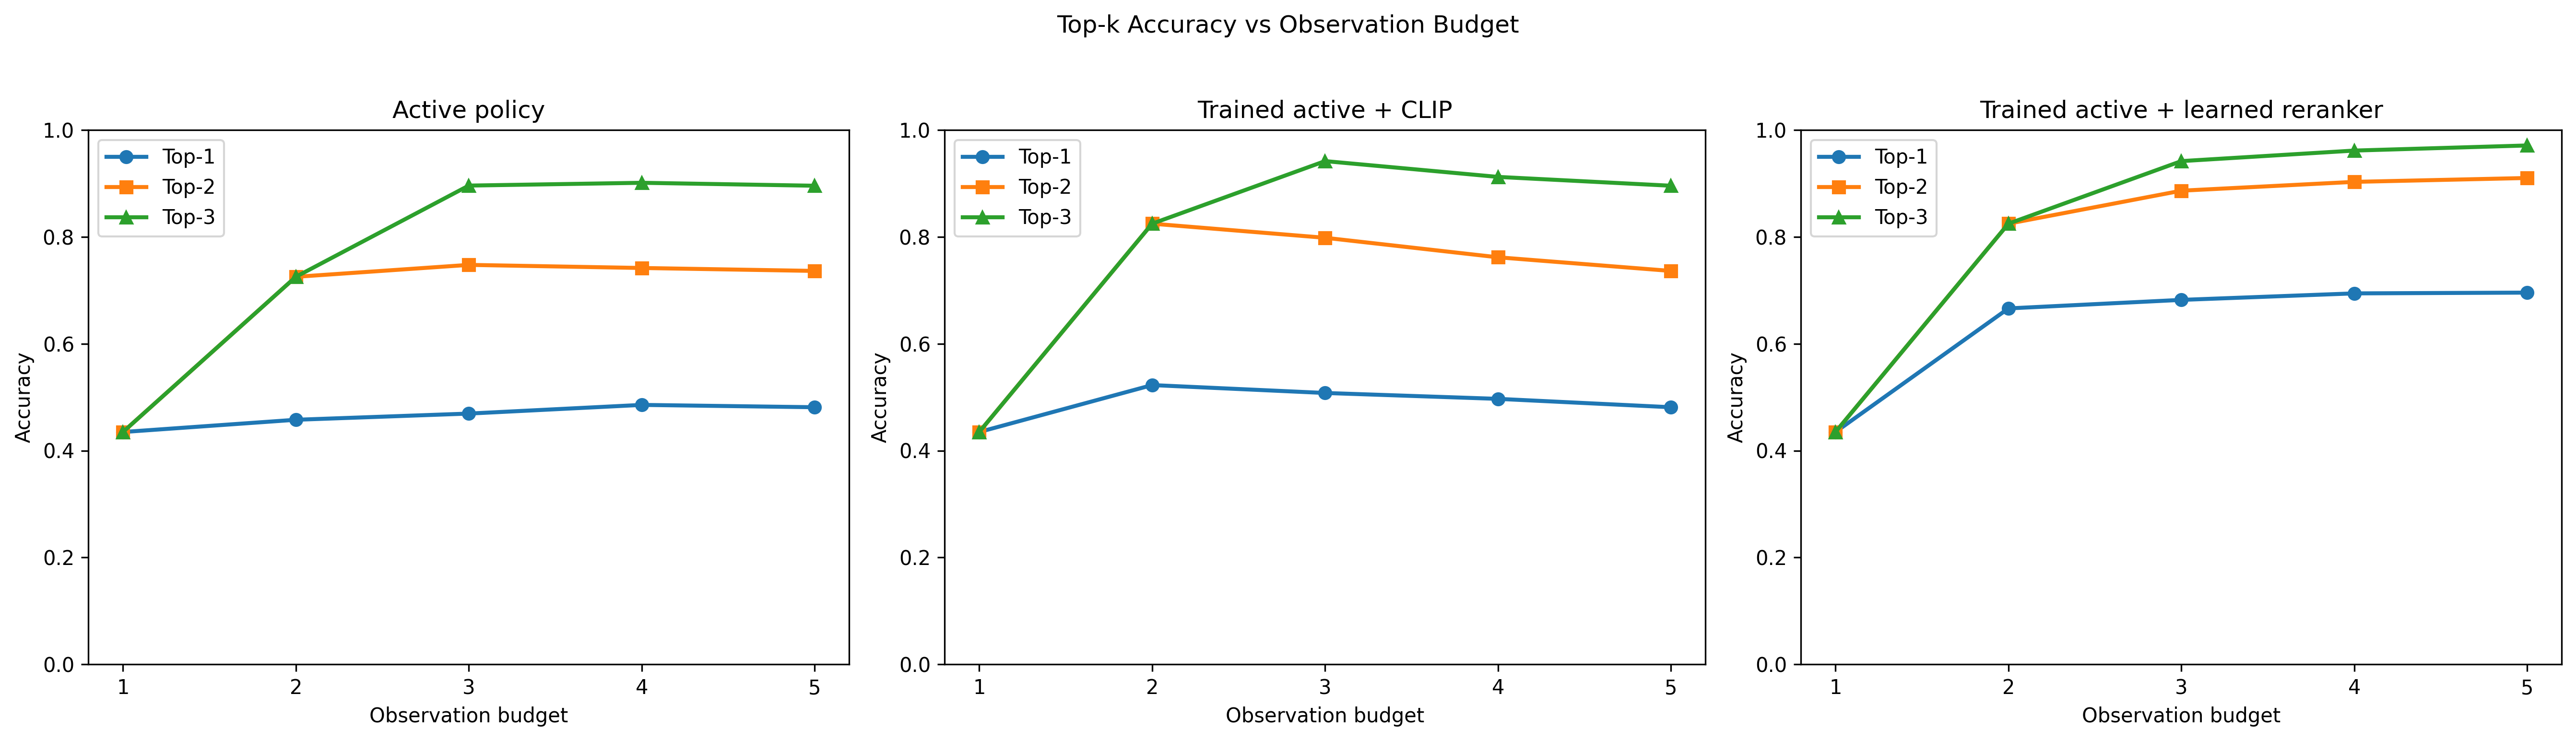
\includegraphics[width=0.95\textwidth]{figures/umd_topk_vs_budget.png}
    \caption{UMD+GT Top-\(k\) accuracy versus budget.
    Top-1 is the final predicted view after selection and ranking; Top-2/Top-3 succeed if a ground-truth view appears among the highest-ranked observed views.}
    \label{fig:umd-topk}
\end{figure}

\subsection{UMD+GT Ablation}

Figure~\ref{fig:umd-ablation-budget3} and Table~\ref{tab:umd-ablation-budget3} report gains versus random-plus-CLIP at budget~3, grouped by affordance.

\begin{figure}[htbp]
    \centering
    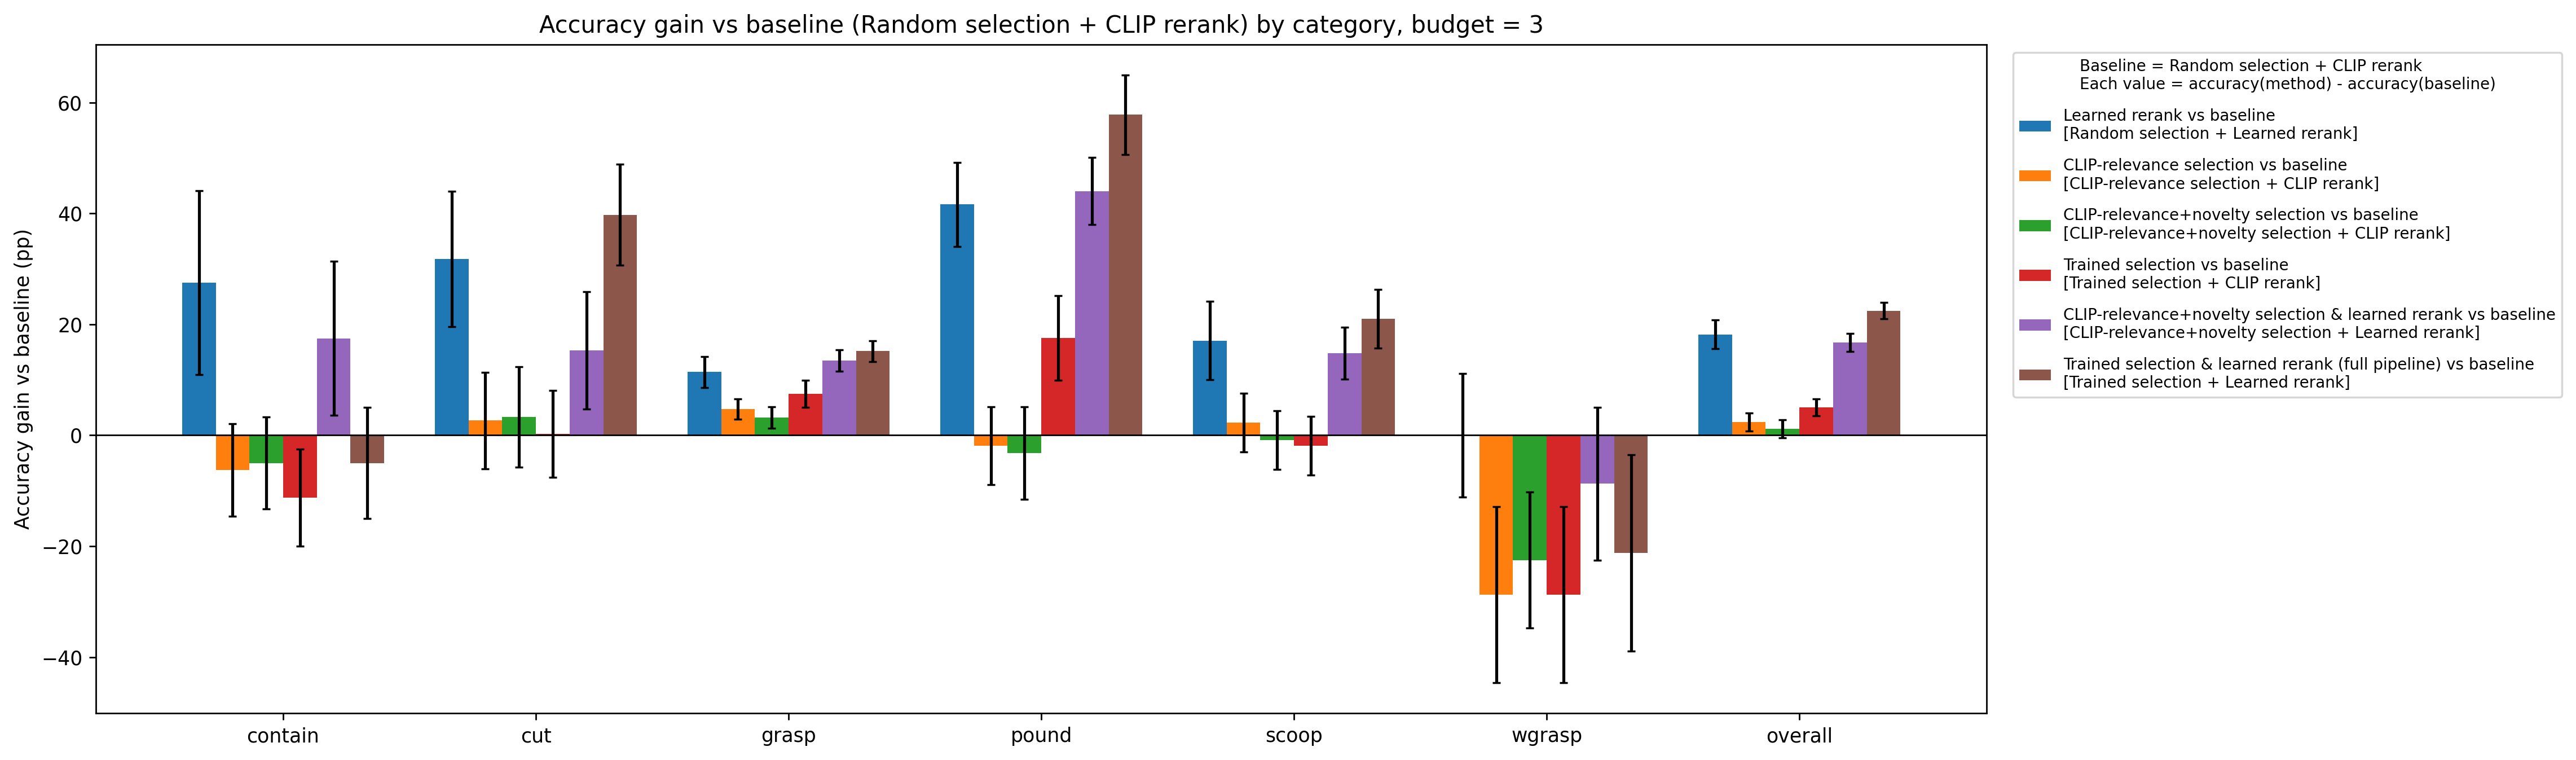
\includegraphics[width=0.95\textwidth]{figures/umd_component_gain_budget_3.png}
    \caption{UMD+GT ablation at budget~3 by affordance.
    Each bar is accuracy(method)~$-$~accuracy(random selection + CLIP rerank).
    Legend entries identify the compared component: learned rerank only, CLIP selection variants,
    trained selection only, combined heuristic selection + learned rerank, and the full pipeline.}
    \label{fig:umd-ablation-budget3}
\end{figure}

\begin{table}[htbp]
    \centering
    \caption{UMD+GT accuracy gain versus random+CLIP at budget~3 (percentage points).}
    \label{tab:umd-ablation-budget3}
    \scriptsize
    \setlength{\tabcolsep}{3pt}
    \begin{tabular}{lrrrrrrr}
        \toprule
        Comparison & cont. & cut & grasp & pound & scoop & wgr. & all \\
        \midrule
        Learned rerank & +27.5 & +31.8 & +11.4 & +41.6 & +17.1 & 0.0 & +18.2 \\
        CLIP-relevance selection & $-$6.2 & +2.7 & +4.7 & $-$1.9 & +2.3 & $-$28.7 & +2.4 \\
        CLIP-rel+novelty selection & $-$5.0 & +3.3 & +3.2 & $-$3.2 & $-$0.8 & $-$22.5 & +1.2 \\
        Trained selection & $-$11.2 & +0.2 & +7.5 & +17.6 & $-$1.9 & $-$28.7 & +5.0 \\
        CLIP-rel+nov + learned & +17.5 & +15.3 & +13.5 & +44.1 & +14.8 & $-$8.8 & +16.8 \\
        Full pipeline & $-$5.0 & +39.8 & +15.2 & +57.8 & +21.0 & $-$21.2 & +22.5 \\
        \bottomrule
    \end{tabular}
\end{table}

\begin{figure}[htbp]
    \centering
    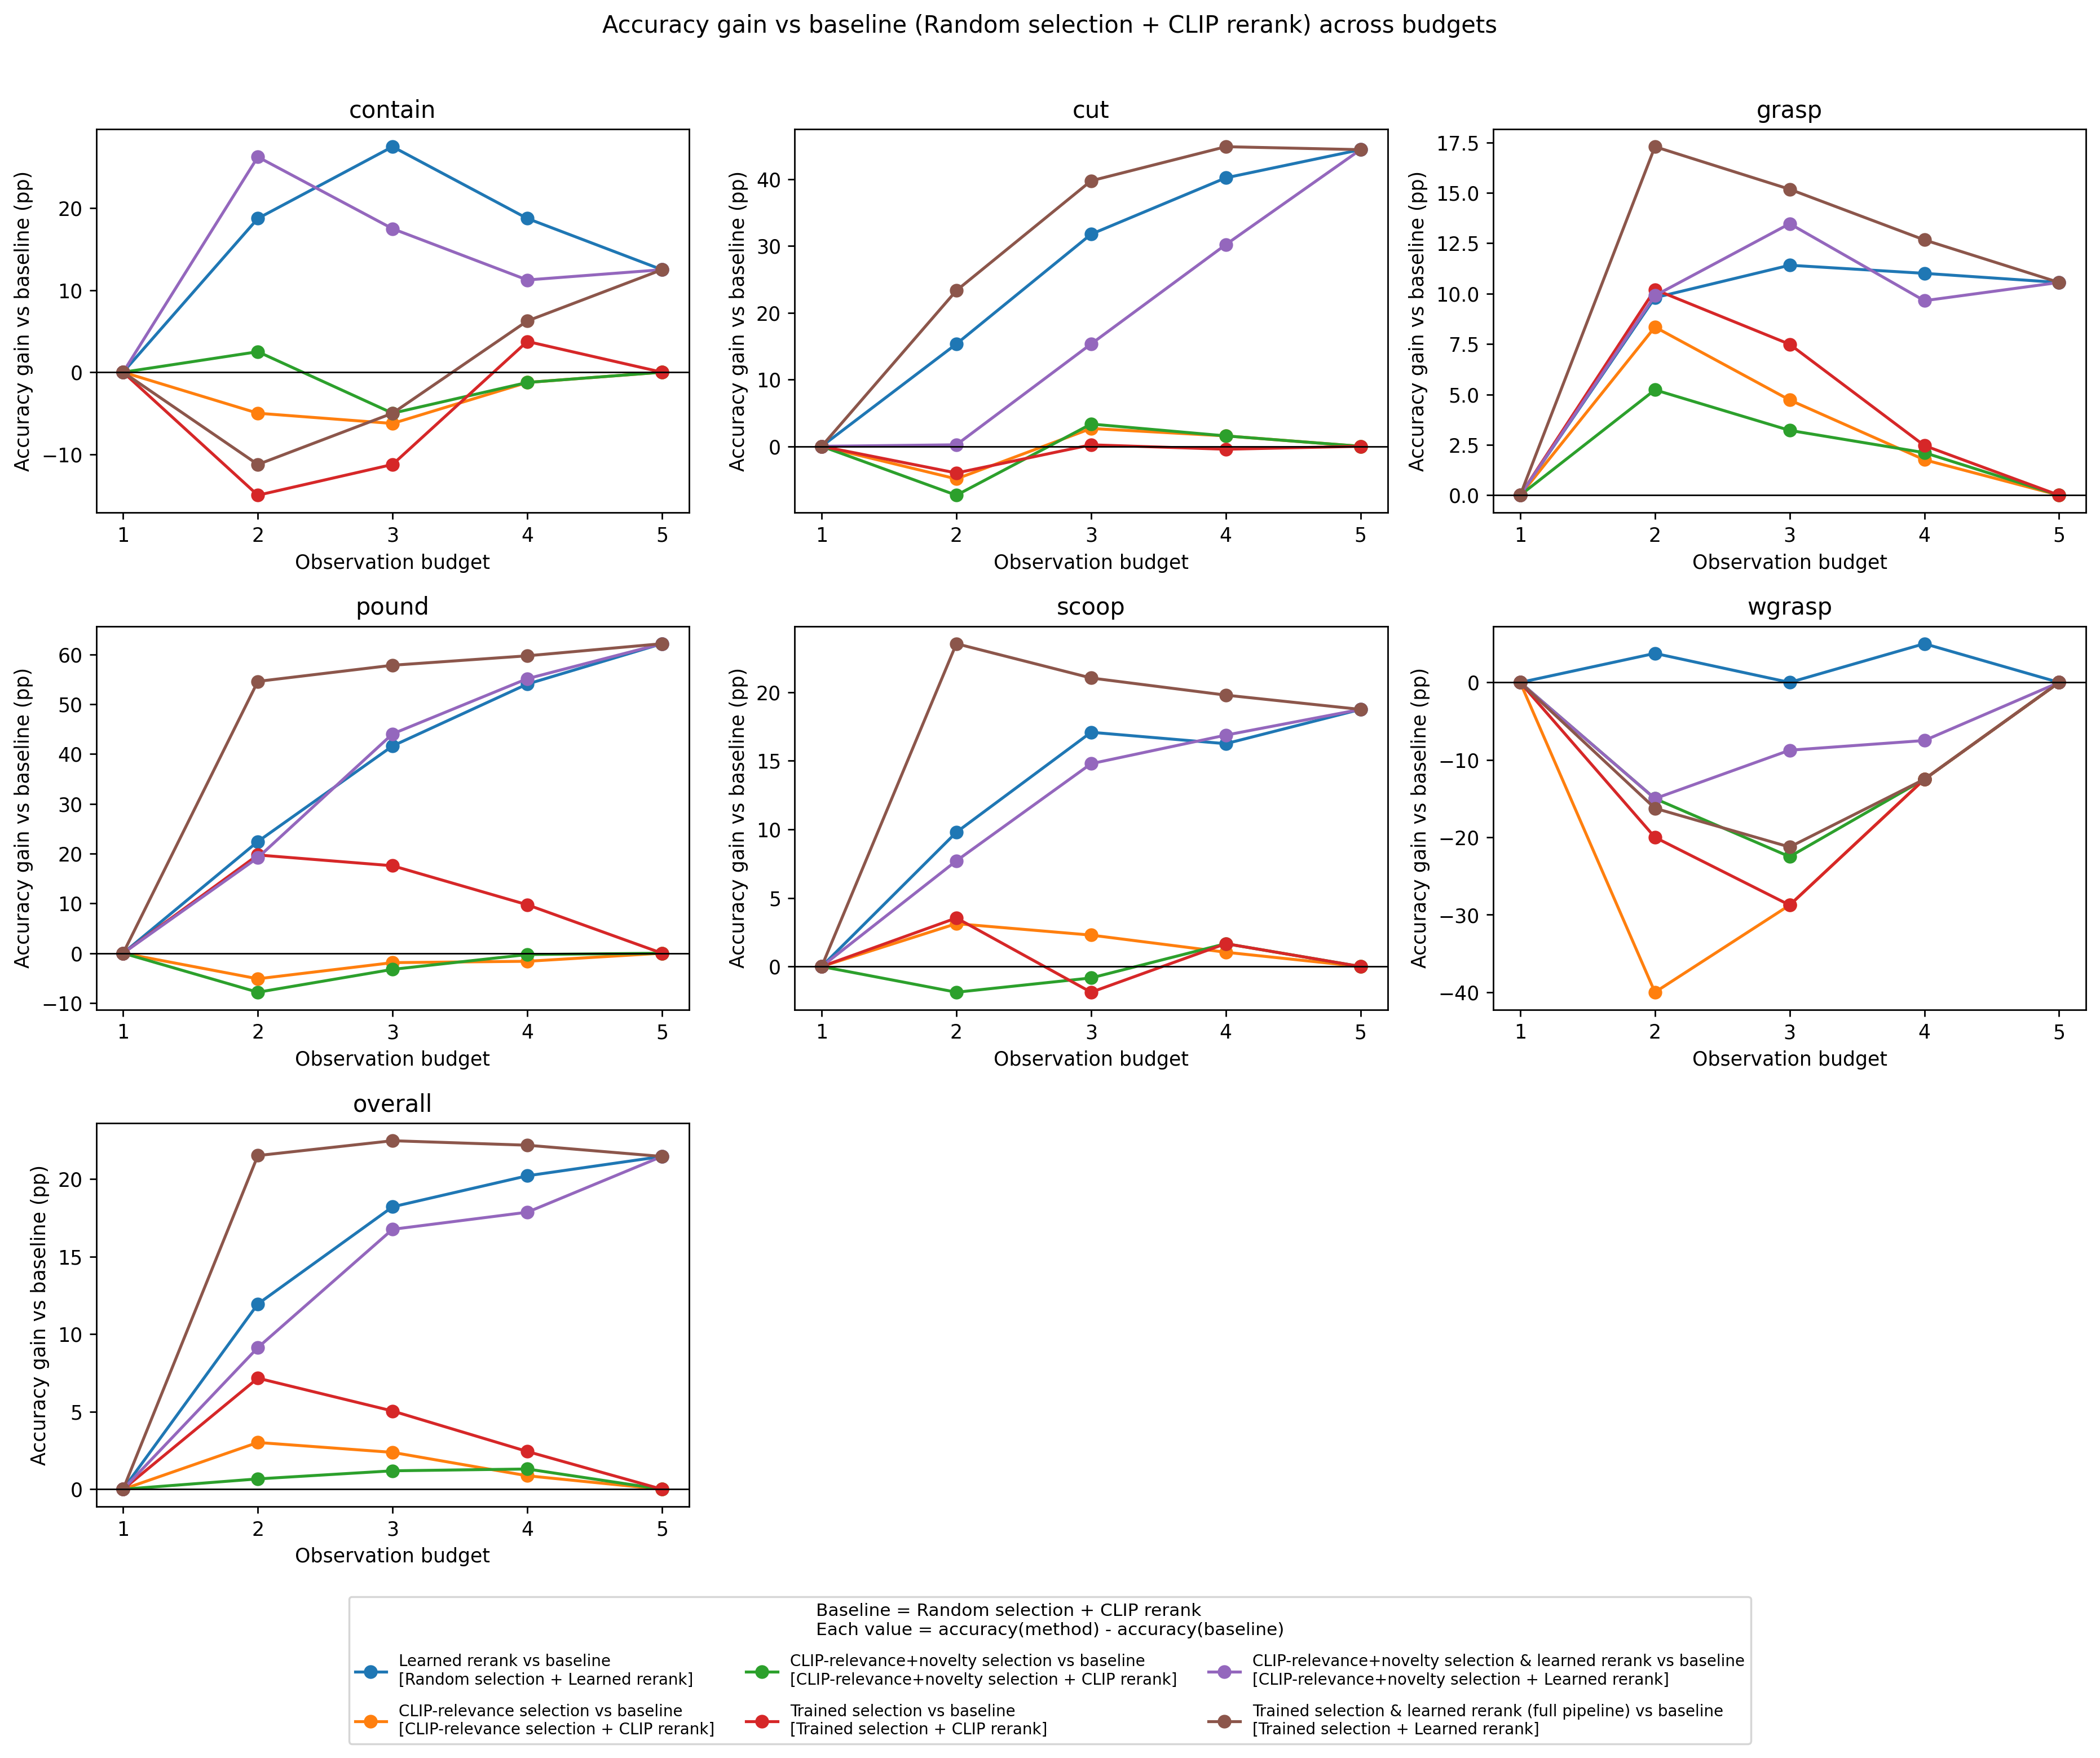
\includegraphics[width=0.95\textwidth]{figures/umd_component_gain_vs_budget.png}
    \caption{UMD+GT component gains versus budget.
    Every curve is accuracy(method)~$-$~accuracy(random+CLIP).
    Positive values mean the named component configuration beats the shared baseline;
    the full pipeline (brown) is strongest at low and medium budgets.}
    \label{fig:umd-ablation-vs-budget}
\end{figure}

The overall ranking at budget~3 is:

\begin{enumerate}
    \item full pipeline: +22.5\,pp;
    \item learned rerank only: +18.2\,pp;
    \item CLIP-rel+nov + learned rerank: +16.8\,pp;
    \item trained selection only: +5.0\,pp;
    \item CLIP selection variants: about +1 to +2\,pp.
\end{enumerate}

Pound, cut, and scoop show the largest gains. Wrap-grasp and contain are noisy or negative for several methods; both have only eight test samples after conversion filters remove rotationally ambiguous cases. By budget~5, all learned-reranker methods converge near +16\,pp overall, again confirming that selection matters mainly when the observation budget is small.

\section{Cross-Dataset Discussion}

Comparing the two datasets yields a consistent pattern and an important difference.

The consistent pattern is that learned reranking is the dominant improvement over CLIP cosine similarity. On both datasets, CLIP-only active policies stay close to exhaustive CLIP, while replacing the final ranker with the MLP produces large gains as soon as two or more views are available.

The important difference is the value of the trained selector. On shuffled CO3D, CLIP relevance-plus-novelty plus learned reranking can match or exceed the full pipeline. On UMD+GT, the full pipeline is clearly best at budgets 2--4. UMD affordance areas change gradually around the turntable, so the selector can learn a more reliable next-view preference. CO3D instructions such as ``front-facing printed design'' are more discrete and category-specific, and the selector/reranker objective overlap is more harmful there.

Another practical observation is that budget~1 is identical for all sequential methods: with only the random initial view, selection never occurs and final ranking has only one candidate. Differences therefore appear from budget~2 onward.

\section{Error Analysis}

Several sources of error remain.

First, CLIP cosine similarity is often too coarse for fine-grained viewpoint differences. Exhaustive CLIP stays near 0.36 on CO3D and 0.48 on UMD+GT, only slightly above chance-aware random baselines.

Second, the selector and reranker are trained with the same binary GT-view objective. This makes them redundant: the selector tends to fetch views that the reranker would already score highly. A selector trained to maximise expected improvement given the current observed set could provide complementary behaviour.

Third, both the heuristic and trained selectors score candidate views using their true image features. In a real robot, those images are unavailable until the camera moves. The reported selection results are therefore an optimistic upper bound relative to pose-only next-best-view prediction.

Fourth, ground-truth definitions remain approximate. On CO3D, labels are instruction-dependent and can be subjective. On UMD+GT, relative mask area is a useful proxy for ``most clearly visible'', but a foreshortened region can cover many pixels without being the most informative view for a human.

Fifth, some groups have few evaluation samples. CO3D categories have 10 evaluation objects each, and UMD contain/wrap-grasp each have only eight test samples. Per-group deltas should therefore be interpreted cautiously.

\section{Summary}

The experiments show that language-guided active view selection is feasible and that a learned MLP on frozen CLIP features substantially improves final view ranking.
On CO3D, learned reranking is the main contributor and the full pipeline helps most at low budgets.
On UMD+GT, over 20 trials, the full trained pipeline is the strongest overall method, reaching \(0.669 \pm 0.011\) at budget~2 and \(0.680 \pm 0.008\) at budget~3 against a random-plus-CLIP baseline near 0.46.
The next chapter discusses these findings, their limitations, and directions for future work.
